\documentclass[a4paper]{article}

\usepackage[english]{babel}
\usepackage[utf8]{inputenc}
\usepackage{amsmath}
\usepackage{graphicx}
\usepackage[colorinlistoftodos]{todonotes}
\usepackage{xeCJK}
\usepackage{setspace}
\usepackage{amsmath}
\usepackage{multirow}
\usepackage{array}
\usepackage{booktabs}
\usepackage{epsfig}
\usepackage{subfigure}
\usepackage{pythonhighlight}
\usepackage{float}
\usepackage{latexsym}
%\setCJKmainfont{SimSun}
\usepackage{geometry}
\geometry{a4paper,left=2.54cm,right=2.54cm,top=2.54cm,bottom=2.54cm}

\title{Notes of Tree Models $\left(\uppercase\expandafter{\romannumeral1}\right)$}
\author{张春光}
\begin{document}
\par\setlength\parindent{1cm}
\maketitle{}
% ============================================================================================================================================
% ============================================================================================================================================
% ============================================================================================================================================
\section{DecisionTree}

	\begin{enumerate}
		\item 基本流程 \par
			决策树的生成是递归产生叶结点的过程, 而产生叶结点主要分为三种情况:
				\begin{itemize}
					\item[(1)] 当前节点包含的样本全部属于同一类别;
					\item[(2)] 当前属性值为空,没有其他属性进行划分,归类为结点中数目最多所属类别;
					\item[(3)] 当前节点包含样本为空,则按照父节点的样本分布作为该结点样本分布;
				\end{itemize}
			\noindent\rule[0.1\baselineskip]{\textwidth}{0.75pt}\\
			\textbf{Decision Tree Pseudo Code}\\
			\noindent\rule[0.1\baselineskip]{\textwidth}{0.5pt}\\
			\textbf{Input:} Train dataset $D = \{(\textbf{x}_i,\,y_i)\,|\,i = 1, 2,\dots, n;\, y_i = 1, 2, ..., k\}$;\\
			\hspace*{32pt} Attributes set $A = \{A_1,A_2,\dots, A_m\}$;\\
			\hspace*{32pt} Threshold $\epsilon$. \par
			\textbf{Procedure:} TreeGenerate($D,\,A$)
				\begin{itemize}
					\item Generate a note N;
					\item \textbf{if} all instance in $D$ belong to a class j \textbf{then}\\
							\hspace*{12pt} Label node N as Leaf Node of class j; \textbf{return}\\
						\textbf{end if}
					\item \textbf{if} $A = \emptyset$ or values of $\textbf{x}_{i}'s$ in $D$ are same \textbf{then}\\
							\hspace*{12pt} Label node N as Leaf Node of the class which has the most instance in $D$; \textbf{return} \\ \textbf{end if}
					\item Select a optimal partitioning attributes $A_*$.(\textbf{ID3,\, C4.5, \, Cart});\\
					\textbf{if} $Gain(D,\,A_*) < \epsilon$; \(OR Gain\_Ratio Or Gini\_Index\); \textbf{return}\\
						\textbf{end if}\\
					\textbf{for} value $a_*^{v}$ in $A_*$:\\
						\hspace*{12pt} Generate branch for N; denote $D_v$ as subsample of $D$ which have value $a_*^{v}$;\\
						\hspace*{12pt} \textbf{if} $D_v$ is empty \textbf{then} \\
							\hspace*{24pt} Label node N as Leaf Node of class j; \textbf{return}\\
						\hspace*{12pt} \textbf{else}\\
						\hspace*{21pt} Denote TreeGenerate($D_v,\, A\backslash{a_*^{v}}$) as child node;\\
						\hspace*{12pt} \textbf{end if}\\
					\textbf{end for}
				\end{itemize}
			\textbf{Output:} An Decision Tree\par
			\noindent\rule[0.1\baselineskip]{\textwidth}{0.75pt}

		从上述伪代码中可以看出,决策树的主要学习内容为属性划分选择,但在实际应用中若决策树结点过多或多少往往会产生过拟合或拟合不足情况,因此较好的决策树需要进行剪枝处理;

		\item 属性划分\par
			决策树的节点优劣常用纯度划分,因此节点属性划分通常以纯度提高来进行衡量,目前纯度常用的衡量指标包括信息增益、信息增益率以及基尼指数;对这三个指标来说,信息增益、增益率指标数值越高,节点属性划分的纯度提升越大, 基尼指数则相反,但这三个指标从原理上来看对于指标选取都是有偏的,其他指标如QUEST算法采用ANOVA选取p值最小的属性进行划分;
			\begin{itemize}

					\item[(1)] 信息熵--倾向多值属性\par
						假设一节点N包含K类样本,记$p_k$为第k类样本的比例,则节点N的信息熵为:
						$$Ent(N) = -\sum_{k=1}^{K}p_klog_2p_k$$ 
						假定离散属性a有V个不同取值,记$N^v$为N中属性a上取值为$a^v$的样本,记$|S|$为样本S的容量,则采取属性a进行划分的信息增益为:
						$$Gain(N,\,a) = Ent(N)-\sum_{v=1}^{V}\frac{|N^v|}{|N|}Ent(N^v)$$
						从信息增益准则公式可以看出\textbf{当样本量不充分大}时,若一个划分属性的取值数目越多,则信息增益会越小,因此信息增益偏好属性取值较多的属性进行划分。

					\item[(2)] 信息增益率--倾向不平衡属性\par
						为消除信息增益准则的偏好性,衍生的$C4.5$算法使用信息增益率为基础计算纯度的提升.
						\begin{align*}
						Gain\_ratio(N,\,a) &= \frac{Gain(N,\,a)}{SplitInformation(N,\, a)}\\
						SplitInformation(N,\, a) &= - \sum_{v=1}^{V}\frac{|N^v|}{|N|}log_2\frac{|N^v|}{|N|}
						\end{align*}
						其中SplitInformation(N,\, a)称为分离信息,一般随着属性a取值个数增多而变大。\textbf{C4.5算法并不直接使用信息增益率来选取属性划分,而是先取信息增益高于平均信息增益的属性,再从其中选择增益率高的属性}.

					\item[(3)] 基尼指数--偏向多值属性\par
						CART(Classification and Regression Tree)可用于分类和回归树,使用基尼指数来选择属性,节点属性衡量方法:
						\begin{align*}
						Gini\_index(N,\,a) &= \sum_{v=1}^{V}\frac{|N^v|}{|N|}Gini(N^v)\\
						Gini(N^v) &= - \sum_{v=1}^{V}\frac{|N^v|}{|N|}log_2\frac{|N^v|}{|N|}
						\end{align*}

					\item[(4)] 其他如$TwoingValue = \frac{|T_L|*|T_R|}{n^2}*(\sum_{v=1}^{V}|\frac{L_i}{|T_L|}-\frac{L_i}{|T_R|}|)^2$等;\par

					\item[(5)] 连续属性\par

						信息熵与基尼指数都是基于离散变量进行计算,而当碰到连续属性时,模型先进行连续数据离散化,$ID3$决策树无法对连续性数据构造决策书,而$C4.5$则基于二分类方法对连续属性进行处理:
							\begin{itemize}
								\item 对属性特征进行排序;
								\item 对于每个特征,有V个特征值,则有V-1个中点值可将数据分为两部分,计算每个中值进行分裂的信息增益;
								\item 选择修正信息增益最大的分裂点作为该属性的划分点对数据划分;
							\end{itemize}
						\begin{align*}
							Gain(N,\,a) & = max_{t\in T_a} Gain(N,\,a,\,t)\\
										& = max_{t\in T_a} (Ent(N) - \sum_{\lambda \in \{-,+\}}\frac{|N_t^\lambda|}{|N|}Ent(N_t^\lambda))\\
									T_a	& = \{\frac{a^i+a^{i+1}}{2}|1\le i \le V-1\}\\
					  GainRevise(N,\,a) & = Gain(N,\,a) - \frac{log_2(V-1)}{|N|}\\
						\end{align*}

			\end{itemize}

		\item 缺失值处理\par
			决策树在学习过程中对缺失值的处理主要从以下两方面:
				\begin{itemize}
					\item 属性选择
						基于每个属性的无缺失样本$\bar{N}$计算信息增益或基尼系数,而后乘以无缺失比例:
						$$Gain(N,\,a) = \rho \times Gain(\bar{N},\,a),\quad \rho = \frac{|\bar{N}|}{|N|}$$
					\item 样本划分
						在基于无缺失的样本属性选择之后,将每个缺失样本按照无缺失样本的后验概率的权重划分入各个子节点中。
				\end{itemize}

		\item 多变量组合属性划分\par
			多变量决策树对于非叶结点划分时是对属性的线性组合进行测试,试图在每次属性划分时建立一个线性分类器。多变量决策树中较为常用的是OC1算法(Oblique Classifier 1);
			大致思想如下:
				\begin{itemize}

					\item[(1)] Coefficients Learning\par
						\begin{itemize}

							\item CART Linear Combination:
								\begin{itemize}
									\item[(1)] 先基于单变量选择最优属性$\textbf{x}_{j.}$,建立多变量组合分割平面H:$\sum_{i=1}^{m}a_ix_i+a_{m+1}=0$
									\item[(2)] 每次基于当前结点数据优化一个$\sum_{i=1}^{m}a_ix_i-\delta(x_i+\gamma)+a_{m+1}<=0(>=0)$,寻求最优$a_i,\,a_{m+1}$使得当前结点内的样本分类正确并更新;
									\item[(3)] Randomization; 因为在步骤(2)中每次更新$a_i$都是局部更新,因此在得到变量组合分割的超平面之后会进行扰动优化,生成
									随机向量$(r_1,r_2,\dots, r_{m+1})$加入超平面使得$H_1 = \sum_{i=1}^{m}(a_i+\alpha r_i)x_i+(a_{m+1}+r_{m+1})$再次优化;
								\end{itemize}

							\item Recursive Least Square procedure
								\begin{align*}
								  W_k &= W_{k-1}-K_k(X_k^TW_{k-1}-y_k)\\
								  K_k &= P_kK_k\\
								  P_k &= P_{k-1} - P_{k-1}X_k[1+X_k^TP_{k-1}X_k]^{-1}X_k^TP_{k-1}
								\end{align*}

						\end{itemize}

					\item[(2)] Feature Selection\par
						特征选取和回归中的stepwise类似采取SBE(Sequential Backward Elimination) 和SFE(Sequential Forward Selection)等, 以SBE为例,对具有
						n个属性的组合寻求最优参数,接下来依次删除其中一个属性,选择精度提高最多的一个属性进行剔除,以此类推,再用独立训练集验证;

				\end{itemize}


		\item 剪枝处理
			机器学习分类方法目的主要是为了提取某一类型样本的一般性特征,提高模型泛化识别能力,而非单一样例的个别特征,因此当决策书模型过深时,所产生的树模型往往会学习到个别特征,因此树模型一般需要进行剪枝处理来防止过拟合现象。
			\begin{itemize}
				\item[(1)] 预剪枝(阈值)\par
					预剪枝即在模型划分前对结点进行估计计算衡量指标,若不能提升则停止进行划分并标记为叶结点;
					预剪枝的优点在于模型训练的成本降低,但决策树训练时很多分支未展开导致存在欠拟合现象。预剪枝一般有以下几种形式:
						\begin{itemize}
							\item 设定决策树最大深度;
							\item 节点中的样本个数小于阈值;
							\item 结点分裂的信息增益小于阈值;
						\end{itemize}

				\item[(2)] 后剪枝(损失函数)\par
					后剪枝即在模型训练生成完整一决策树时从下而上,对非叶结点进行替换为叶结点计算模型的泛化能力,若有提升则将将该结点替换为叶结点进行。
				从原理上来看,预剪枝寻求局部优化,而后剪枝以成本开销为代价寻求全局优化。预剪枝一般在模型构建中使用阈值来处理,而后剪枝一般使用树损失函数来进行剪枝;
							
			\end{itemize}

		\item 三种决策树算法
			决策树算法主要分为二叉树与多叉树模型,前者代表有CART和QUEST算法,后者有FACT、C4.5、CHAID、FRIM算法等, 这里主要介绍ID3、C4.5及CART算法;
			\begin{itemize}

				\item[(1)] ID3 决策树\par
					最早的决策树类型,采用信息增益指标进行评估和特征选择,也较为粗糙。
					\begin{itemize}
						\item 只能处理离散属性,无法处理连续属性;
						\item 只生成树,未进行后剪枝处理;
						\item 信息增益准则偏好取值数目较多的属性;
						\item 适用于小规模数据集。
					\end{itemize}

				\item[(2)] C4.5 决策树\par
					C4.5决策树继承ID3决策树并进行改进:
					\begin{itemize}
						\item 结合信息增益和信息增益率进行属性划分选择,避免偏好取值多的属性;
						\item 使用二分法对连续属性离散化处理,对离散属性则采用多分法; 
						\item 有对缺失值进行处理;
						\item 可以在树构造过程中进行剪枝(信息增益率阈值等),采用悲观剪枝法(Pessimistic Error Pruning);
							\begin{itemize}
								\item 对任意结点t, 假设结点的样本个数为$N(t)$, 该结点根据最优属性划分为$N_t$;
								\item 计算将结点t作为叶结点的错误率$error_t = n(t) +\frac{1}{2}$;
								\item 计算将结点作为内部结点的错误率 $error_{T_t} = n(T_t)+\frac{N_t}{2}$以及标准差$SE = \sqrt{\frac{n(T_t)(N(t)-n(T_t))}{N(t)}}$
								\item 若$error_{T_t}+SE - error_t>0$,则将结点t作为叶结点,反之不剪枝;
							\end{itemize} 
						\item \textbf{由于在构造树时需要对数据的属性进行多次扫描和排序,占内存、低效}
					\end{itemize}
					目前基于C4.5的基础上产生了C5.0算法,可应用于大数据集,采用Boosting方式提高模型准确率,又成为BoostingTrees, 占用内存少,速度较快;
					但其本质上不是单决策树而是基于决策树的集成方法;
					%CHAID算法是在C4.5的算法基础上增加一步合并某些结点;
					FIRM算法则是在CHAID算法上每个连续性属性划分为10个属性在进行树的生成, 但不进行剪枝;

				\item[(3)] CART 分类树\par
					CART决策树为分类与回归树,假定决策树是二叉树,内部结点特征为是和否,递归二分每个特征,在进行回归时使用叶结点的样本的均值输出预测值;
					\begin{itemize}
						\item 使用GINI系数进行属性划分;
						\item 对于连续属性采用多次二分法,离散属性划分时每次选择其中一种分割数据,对属性特征重复性使用;
						\item 对于多分类目标,会将目标类别合并成两个超类别;
						\item 对于树的构建,CART算法会生成尽量大的数目,而后用验证数据集根据损失函数对已生成的树进行剪枝,选择最优子树;
						\item 采用独立的验证集剪枝处理,否则剪枝结果为深度最大的子树;
							\begin{itemize}
								\item 对整棵树分别计算以内部结点t为单结点的树(t)和根节点的树($T_t$)的损失函数
									$$C_\alpha(t) = C(t)+\alpha,\quad C_\alpha(T_t) = C(T_t)+\alpha|T_t|$$
								\item 当且仅当$C_\alpha(t)<C_\alpha(T_t)$时,决策树会进行剪枝剪除$T_t$
								\item 令$g(t) = \frac{C(t)-C(T_t)}{|T_t|-1}$,计算所有内部结点t的g(t)值,依次增加$\alpha$,自下而上地在$T_i$中剪除g(t)最小的$T_(t)$得到
								$T_{i+1}$子树
								\item 利用独立测试集计算独立子树的损失函数,取最优子树.
							\end{itemize}
						\begin{align*}
								C_{\alpha}(T) & = C(T) + \alpha\|T\|\\
											& = \sum_{t=1}^{|T|}N_tH_t + \alpha\|T\|\\
										H_t	& = -\sum_k\frac{N_{tk}}{N_t}log\frac{N_{tk}}{N_t}
							\end{align*}
						$\alpha$为树模型复杂度的惩罚系数, $\|T\|$为树的叶结点数目, $N_t$为叶结点t上的样本数,$N_{tk}$为叶结点t上为类k的样本数;$H_t$为叶结点t上的经验熵;	
					\end{itemize}
					\textbf{CART回归树}主要先将输入空间划分为M个空间$R_1,R_2,\dots,R_M$, 每个空间对应输出值$c_1,c_2,\dots,c_M$,而在对属性A选择和切分点v时不是选择
					信息增益或基尼指数,而是最小化:
					$$min_{A,s}[min_{c_1}\sum_{x_i\in \{x|x^A\leq s\}}(y_i-c_1)^2+min_{c_2}\sum_{x_i\in \{x|x^A\geq s\}}(y_i-c_2)^2]$$.
					其中$c_i$在平方误差损失函数下一般取值为$R_i$区间内样本的均值;

				\item[(4)] Scikit\-learn 模块中使用的决策树算法为CART算法;\par
					$DecisionTreeClassifier(criterion='gini',\, splitter='best',\, max\_depth=None, \\
					\hspace*{12pt}min\_samples\_split=2,\, min\_samples\_leaf=1,\, min\_weight\_fraction\_leaf,\\
					\hspace*{12pt}max\_features=None,\, random\_state=None,\, max\_leaf\_nodes=None, \\
					\hspace*{12pt}min\_impurity\_decrease=0.0,\, min\_impurity\_split=None,\\
					\hspace*{12pt}class\_weight=None,\, presort=False)$
			\end{itemize}
	\end{enumerate}
% ============================================================================================================================================
% ============================================================================================================================================
% ============================================================================================================================================
\section{Bagging}
% ============================================================================================================================================
	\subsection{RandomTreesEmbedding}
		\begin{align*}
			Dataset D & \Rightarrow Bootstrap m subdataset(D_1, D_2,\dots, D_m)\\
					  & \Rightarrow Train m learner {I_i(x_i)}\\
					  & \Rightarrow H(x) = argmax \sum_{m=1}^{M}I(I_t(x)=y)
		\end{align*}
		Bagging结合Bootstrap,使得模型有部分验证集对组合学习器进行包外估计,可以起到降低方差的效果, 不易受干扰.
% ============================================================================================================================================
	\subsection{RandomForest}
	随机森林在RandomTreesEmbedding上基础上进行改进,在构建每克决策树过程中引入\textbf{随机属性选择}.传统决策树在选择属性划分时候对当前结点的属性集合(d)中
	选择最优属性,而在随机森林中,先对当前结点的属性集合中随机选择k(一般$k = log_2d$)个属性子集,然后再从属性子集中选择最优属性。
% ============================================================================================================================================
	\subsection{StackingStrategy}
		Average, WeightedAverage, Majority Vote, MetaLearnerStacking,\dots
% ============================================================================================================================================		
\section{Boosting}
	\begin{itemize}
		\item[(1)] Boosting 基本流程:
			\begin{itemize}
				\item 从初始训练集用初始权重训练出一个基学习器$h_1$;
				\item 根据基学习器的学习误差率$\epsilon$表现更新训练样本权值,使得误差率高的训练样本权值$W_i$增加;
				\item 基于新的样本权值训练基学习器$h_2$;
				\item 迭代进行,直到基学习器数目到达预设数目T,然后根据基学习器的权重$\alpha_i$组合基学习器的训练结果输出;
				\begin{figure*}[h]
					\centering
					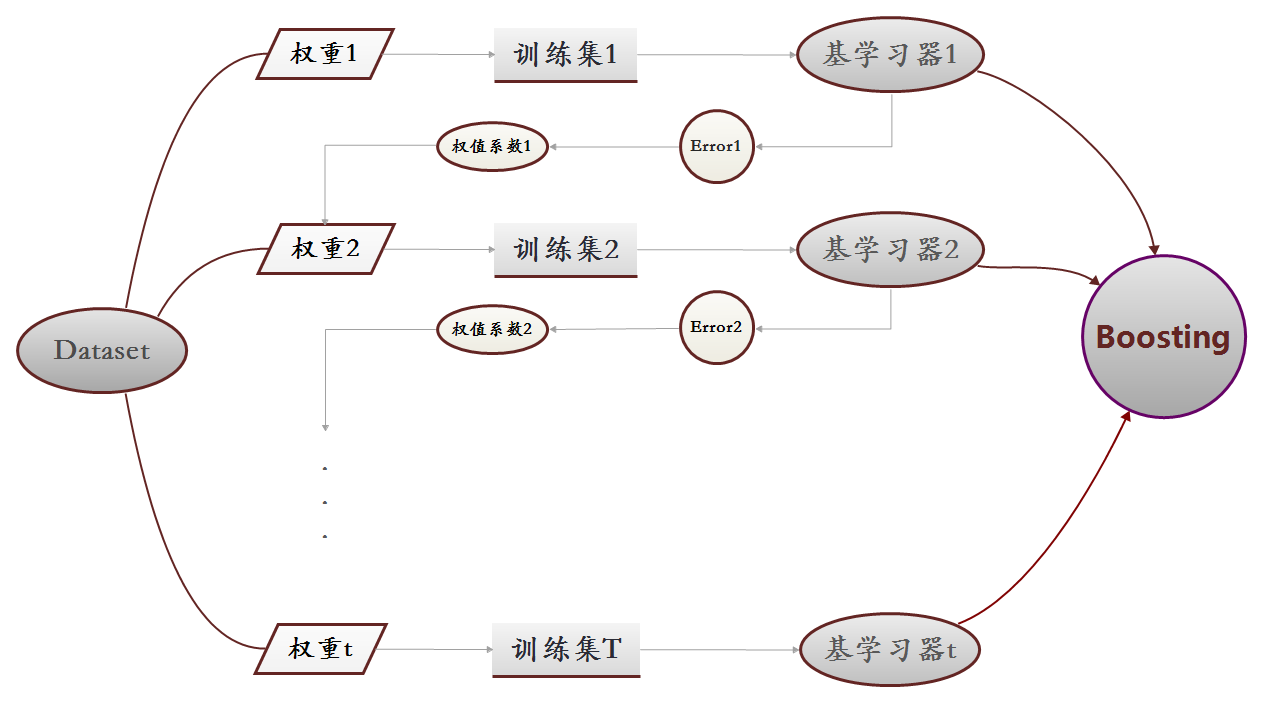
\includegraphics[width=0.9\textwidth]{Dataset.png}
					\caption{Boost}
				\end{figure*}
			\end{itemize}
			所以不同的Boosting方法的区别在于以下几点:
			\begin{itemize}
				\item 学习误差率的计算方式Loss function;
				\item 如何根据误差率更新样本权重系数W;
				\item 如何确定基学习器的权重系数(如何组合基学习器);
			\end{itemize}
			针对大部分Boosting算法,基本都是采用加法模型来组合弱分类器,用前向分布算法来改变训练数据的权重和概率分布;

		\item[(2)] 加法模型Additive model
			\begin{itemize}
				\item 考虑由K棵树组成加法模型:$$\hat{y} = \sum_{k=1}^{K}\beta_{k}f(x)$$
				\item 解决这一优化问题可采用前向分布算法从前往后每次只学习一个基函数及其系数,逐步逼近优化目标函数来简化复杂度,即
				$$Obj^{(t)} = \sum_{i=1}^{n}l(y_i, \hat{y}_i^t)+\sum_{i=1}^{t}\Omega(f_i) = \sum_{i=1}^{n}l(y_i, \hat{y}_{i}^{t-1}+f_t(x_i))+\Omega(f_t)+constant$$
				\item 因此,最优化目标函数就转化为基于前一学习器的预测来最优化当前损失函数,即最小化$\sum_{i=1}^{n}l(y_i, \hat{y}_{i}^{t-1}+f_t(x_i))+\Omega(f_t)$;
				\item 以平方损失函数为例,则模型转为拟合上一轮的残差$$\sum_{i=1}^{n}(y_i-\hat{y}_{i}^{t-1}+f_t(x_i))^2+\Omega(f_t) = \sum_{i=1}^{n}(\epsilon_i - f_i(x))^2 + \Omega(f_t)$$
				\item 而损失函数的形式及其泰勒展开项数的不同产生就衍生出不同的Boosting算法;
			\end{itemize}
	\end{itemize}
% ============================================================================================================================================
% ============================================================================================================================================
	\subsection{AdaBoost}
		\subsubsection{AdaBoost}
			AdaBoost采用损失函数为最小化指数损失函数$l_{exp}(H|D)$的线性[权重]加法\textbf{前向分布算法}模型输出H(x),假定f为真实分布,即
				\begin{align*}
					H(\textbf{x}) & = \sum_{t=1}^{T}\alpha_th_t(\textbf{x})\\
			   		l_{exp}(H|W)& = E_{\textbf{x}|W}[exp(-f(x)H(x))]
				\end{align*}

			\noindent\rule[0.1\baselineskip]{\textwidth}{0.75pt}\\
			\textbf{Algorithm: AdaBoost for Binary Classification}\\
			\noindent\rule[0.1\baselineskip]{\textwidth}{0.5pt}\\
			\textbf{Input:} Train dataset $D = \{(\textbf{x}_i,\,y_i)\,|\,i = 1, 2,\dots, n;\, y_i = -1, 1\}$;\\
			\hspace*{32pt} WeakLearn Algorithm I;\\
			\hspace*{32pt} Number of Weak Learn Algorithm T.\\
			\textbf{Procedure:} 
					\hspace*{2pt} Initializing sample weight vector $W_1(\textbf{x}) = \frac{1}{n}$;\par
					\hspace*{32pt} \textbf{for} $t = 1, 2,\dots, T$ \textbf{do}\par
							\hspace*{48pt} $h_t = I(D, W_t)$;\par
							\hspace*{48pt} $\epsilon_t = P_{\textbf{x}|W_t}(h_t(\textbf{x}) \neq f(\textbf{x}))$;\par
							\hspace*{48pt} \textbf{if} $\epsilon_t > 0.5$ \textbf{then break}\par
							\hspace*{48pt} $\alpha_t = \frac{1}{2}ln(\frac{1-\epsilon_t}{\epsilon_t})$;\par
							\hspace*{48pt} $W_{t+1} = \frac{W_t(\textbf{x})}{Z_t}exp(-\alpha f(\textbf{x})h_t(\textbf{x}))$\par
					\hspace*{32pt}\textbf{end for}\\
			\textbf{Output:} $H(\textbf{x}) = sign(\sum_{t=1}^{T}\alpha_th_t(\textbf{x}))$\par
			\noindent\rule[0.25\baselineskip]{\textwidth}{0.75pt}\par
				\begin{itemize}
					\item[(\romannumeral1)] 样本权值更新方式: $W_t$
											\begin{align*}
												W_{t+1} & = \frac{W_t(\textbf{x})}{Z_t}\times \left \{\begin{array}{ll}
															 					 					exp(-\alpha_t),\, & if\, h_t(x)=f(x);\\
															 					 				    exp(\alpha_t),\, & if\, h_t(x)\neq f(x).
															 					 			 		\end{array} \right. \\
														  & = \frac{W_t(\textbf{x})}{Z_t}exp(-\alpha f(\textbf{x})h_t(\textbf{x}))
										   \end{align*}
					\item[(\romannumeral2)] 损失函数最小化:H(x)
						\begin{align*}
							\frac{\partial l_{exp}(H|W)}{\partial H(\textbf{x})} & = -exp(H(\textbf{x}))P(f(x)=1|x)+exp(H(x))P(f(x)=-1|x)=0\\
																   H(\textbf{x}) & = \frac{1}{2}ln\frac{P(f(x)=1|x)}{P(f(x)=-1|x)}\\
															 sign(H(\textbf{x})) & = sign(\frac{1}{2}ln\frac{P(f(x)=1|x)}{P(f(x)=-1|x)}) \\
															 					 & = \left \{\begin{array}{ll}
															 					 				1,\, &$P(f(x)=1|x) > P(f(x)=-1|x)$;\\
															 					 				-1,\, &$P(f(x)=1|x) < P(f(x)=-1|x)$.
															 					 			 \end{array} \right.\\
															 					 & = arg max_{y\in \{-1,1\}} P(f(x)=y)
						\end{align*}
					\item[(\romannumeral3)] 损失函数最小化:$\alpha_t$
						\begin{align*}
							l_{exp}(\alpha_t h_t|W_t) & = E_{x|W_t}[exp(-f(x)\alpha_th_t(x)] \\
												 & = E_{x|W_t}[e^{-\alpha_t}I(f(x)=h_t(x))+e^{\alpha_t}I(f(x)\neq h_t(x))] \\
												 & = e^{-\alpha_t}(1-\epsilon_t) + e^{\alpha_t}\epsilon_t\\
							\frac{\partial l_{exp}(\alpha_th_t)}{\partial \alpha_t} & = -e^{-\alpha_t}(1-\epsilon_t) + e^{\alpha_t}\epsilon_t = 0 \\
										\alpha_t & = \frac{1}{2}ln\frac{1-\epsilon_t}{\epsilon_t}
						\end{align*}
					\item[(\romannumeral4)] 损失函数最小化[原理类似加法模型]:$h_t$,W(x)
						\begin{align*}
							h_t(x) & = argmin_h l_{exp}(H_{t-1}+\alpha_th(x)|W) \\
								   & = argmin_h E_{x|W}[exp(-f(x)H_{t-1})exp(-f(x)\alpha_th(x))]\\
								   & = argmin_h E_{x|W}[exp(-f(x)H_{t-1})exp(-f(x)h(x))]\\
								   & \equiv argmin_h E_{x|W}[exp(-f(x)H_{t-1})(1-f(x)h(x) + \frac{f^2(x)h^2(x)}{2})]\\
								   & = argmin_h E_{x|W}[exp(-f(x)H_{t-1})(1-f(x)h(x) + \frac{1}{2})] \\
								   & = argmax_h E_{x|W}[\frac{exp(-f(x)H_{t-1})}{E_{x|W}[exp(-f(x)H_{t-1}(x))]}f(x)h(x)] \\
								   & = argmax_h E_{x|W_t}[f(x)h(x)], \, where,\, W_t(x) = \frac{exp(-f(x)H_{t-1})}{E_{x|W}[exp(-f(x)H_{t-1}(x))]} \\
								   & = argmax_h E_{x|W_t}[1-2I(f(x)\neq h(x))] = argmin_h E_{x|W_t}[I(f(x)\neq h(x))]\\
						   W_{t+1} & = \frac{W_texp(-f(x)H_t(x))}{E_{x|W}[exp(-f(x)H_t(x))]} \\
						   		   & = W_texp(-f(x)\alpha_th_t)\frac{E_{x|W}[exp(-f(x)H_{t-1}(x))]}{E_{x|W}[exp(-f(x)H_t(x))]}
						\end{align*}
				\end{itemize}
			AdaBoost作为弱分类器的组合器,基分类器越弱,效果提升越明显,结果也越好,且不容易过拟合,但由于AdaBoost的权值更新方式的原理,AdaBoost对异常数据比较敏感,因异常数据在权值更新中往往会获得较高的权值;
% ============================================================================================================================================
% ============================================================================================================================================	
		\subsubsection{AdaBoost.m1}

			AdaBoost基本算法应用限制在二分类中,而衍生的AdaBoost.m1 是基于AdaBoost的多分类方法,主要区别在于多分类问题在更新权值时,分类错误的样本权值不进行更新,而若分类正确的样本其权重乘以$\frac{\epsilon_t}{1-\epsilon_t}<1$来提高错误分类的样本,其基本算法如下:\par
			\noindent\rule[0.1\baselineskip]{\textwidth}{0.75pt}\\
			\textbf{AdaBoost.m1 for Multiclass Classification}\\
			\noindent\rule[0.1\baselineskip]{\textwidth}{0.5pt}\\
			\textbf{Input:} Train dataset $D = \{(\textbf{x}_i,\,y_i)\,|\,i = 1, 2,\dots, n;\, y_i = 1,2,\dots, k\}$;\\
			\hspace*{32pt} WeakLearn Algorithm I;\\
			\hspace*{32pt} Number of Weak Learn Algorithm T.\\
			\textbf{Procedure:} 
					\hspace*{2pt}Initializing sample weight vector $W_1(\textbf{x}) = \frac{1}{n}$;\par
					\hspace*{32pt} \textbf{for} $t = 1, 2,\dots, T$ \textbf{do}\par
							\hspace*{48pt} $h_t = I(D, W_t)$;\par
							\hspace*{48pt} $\epsilon_t = P_{\textbf{x}|W_t}(h_t(\textbf{x}) \neq f(\textbf{x}))$;\par
							\hspace*{48pt} \textbf{if} $\epsilon_t > 0.5$ \textbf{then break}\par
							\hspace*{48pt} $\beta_t = \frac{\epsilon_t}{1-\epsilon_t}$;\par
							\hspace*{48pt} $W_{t+1} = \frac{W_t}{Z_t}\beta_t^{1-[h_t(\textbf{x})\neq y]}$\par
					\hspace*{32pt}\textbf{end for}\par
			\textbf{Output:} $H(\textbf{x}) = argmax_{y\in C}\sum_{t=1}^{T}ln\frac{1}{\beta_t}[h_t(\textbf{x})=y]$\par
			\noindent\rule[0.1\baselineskip]{\textwidth}{0.75pt}\par

		\subsubsection{AdaBoost.m2}

			AdaBoost.m2 也是基于AdaBoost的多分类方法,不仅关注样本分类是否错误,而且关注样本分类错误是在错分在哪一类别上,因此在更新权值时会更新错误分类的权值(如下所示在更新$\epsilon$时更新$\beta$进而提高错误分类样本的权重,同时在最后一步更新$\omega$是降低修改其他类的权重);\\
			\noindent\rule[0.1\baselineskip]{\textwidth}{0.75pt}\\
			\textbf{AdaBoost.m2 for Multiclass Classification}\\
			\noindent\rule[0.1\baselineskip]{\textwidth}{0.5pt}\\
			\textbf{Input:} Train dataset $D = \{(\textbf{x}_i,\,y_i)\,|\,i = 1, 2,\dots, n;\, y_i = 1,2,\dots, k\}$;\\
			\hspace*{32pt} WeakLearn Algorithm I;\\
			\hspace*{32pt} Number of Weak Learn Algorithm T.\\
			\textbf{Procedure:} 
					\hspace*{2pt} Initializing sample weight vector $W_1(i) = \frac{1}{n}$;\par
					\hspace*{36pt}$\omega_{i,y}^1 = \frac{W_i}{k-1}$ for $i = 1, 2, \dots, n;\quad y\in \{1,2,\dots,k\}\slash{y_i}$; \par
					\hspace*{32pt} \textbf{for} $t = 1, 2,\dots, T$ \textbf{do}\par
							\hspace*{48pt} $\Omega_i^t = \sum_{y\neq y_i}\omega_{i,y}^t$;\par
							\hspace*{48pt} $q_t(i,\,y) = \frac{\omega_{i,y}^t}{\Omega_i^t}\,for\,y\neq y_i$;\par
							\hspace*{48pt} $W_t^i = \frac{\Omega_i^t}{\sum_{i=1}^{N}\Omega_i^t}$;\par
							\hspace*{48pt} $h_t = I(D, W_t)$;\par
							\hspace*{48pt} $\epsilon_t = \frac{1}{2}\sum_{i=1}^{N}W_t(i)(1-h_i(x_i, y_i)+\sum_{i,y\neq y_i}q_t(i,y)h_t(x_i,y))$;\par
							\hspace*{48pt} \textbf{if} $\epsilon_t > 0.5$ \textbf{then break}\par
							\hspace*{48pt} $\beta_t = \frac{\epsilon_t}{1-\epsilon_t}$;\par
							\hspace*{48pt} $\omega_{i,y}^{t+1} = \omega_{i,y}^{t+1}*\beta_t^{\frac{1}{2}(1+h_t(x_i,y_i)-h_t(x_i,y)}$ for $y\in \{1,2,\dots,k\}\slash{y_i}$;\par
					\hspace*{32pt}\textbf{end for};\par
			\textbf{Output:} $H(\textbf{x}) = argmax_{y\in C}\sum_{t=1}^{T}ln\frac{1}{\beta_t}h_t(x,y)$;\par
			\noindent\rule[0.1\baselineskip]{\textwidth}{0.75pt}\par
% ============================================================================================================================================
% ============================================================================================================================================
		\subsubsection{AdaBoost.R}

			AdaBoost.R算法是AdaBoost算法应用于回归问题的改进,但在使用标准AdaBoost.R算法会先将response variable映射在$[0,1]区间内$;\par
			\noindent\rule[0.1\baselineskip]{\textwidth}{0.75pt}\\
			\textbf{AdaBoost.R for Regression Problem}\\
			\noindent\rule[0.1\baselineskip]{\textwidth}{0.5pt}\\
			\textbf{Input:} Train dataset $D = \{(\textbf{x}_i,\,y_i)\,|\,i = 1, 2,\dots, n;\, y_i \in [0,\,1]\}$;\\
			\hspace*{32pt} WeakLearn Algorithm I;\\
			\hspace*{32pt} Number of Weak Learn Algorithm T.\\
			\textbf{Procedure:} 
					\hspace*{2pt} Initializing sample weight vector $W_1(i) = \frac{1}{n}$;\par
					\hspace*{36pt}$\omega_{i,y}^1 = \frac{W_i*|y-y_i|}{Z}$, where $Z = \sum_{i=1}^{n}W(i)\int_{0}^{1}|y-y_i|dy$; \par
					\hspace*{32pt} \textbf{for} $t = 1, 2,\dots, T$ \textbf{do}\par
							\hspace*{48pt} $W^t = \frac{\omega^t}{\sum_{i=1}^{n}\int_{0}^{1}\omega_{i,y}^t}dy$;\par
							\hspace*{48pt} $h_t = I(D, W_t)$;\par
							\hspace*{48pt} $\epsilon_t = \sum_{1}^{n}|\int_{y_i}^{h_t(x_i)}W_{i,y}^{t}|dy$;\par
							\hspace*{48pt} \textbf{if} $\epsilon_t > 0.5$ \textbf{then break}\par
							\hspace*{48pt} $\beta_t = \frac{\epsilon_t}{1-\epsilon_t}$;\par
							\hspace*{48pt} $\omega_{i,y}^{t+1} = \omega_{i,y}^{t}\beta_t^{1-I(y in [y_i, h_t(x_i)])-I(y in [h_t(x_i),y_i])} $;\par
					\hspace*{32pt}\textbf{end for};\par
			\textbf{Output:} $H(\textbf{x}) = inf \{y:\sum_{t:h_t(y)\leq y}log(\frac{1}{\beta_t}\geq \frac{1}{2}log\frac{1}{\beta_t}\}$;\par
			\noindent\rule[0.1\baselineskip]{\textwidth}{0.75pt}
% ===============================================================================================================================================
		\subsubsection{AdaBoost.R2}

			AdaBoost.R2算法是AdaBoost算法应用于回归问题的改进,但在使用标准AdaBoost.R算法会先将response variable映射在$[0,1]$区间内;\par
			\noindent\rule[0.1\baselineskip]{\textwidth}{0.75pt}\\
			\textbf{AdaBoost.R2 for Regression Problem}\\
			\noindent\rule[0.1\baselineskip]{\textwidth}{0.5pt}\\
			\textbf{Input:} Train dataset $D = \{(\textbf{x}_i,\,y_i)\,|\,i = 1, 2,\dots, n;\, y_i \in [0,\,1]\}$;\\
			\hspace*{32pt} WeakLearn Algorithm I;\\
			\hspace*{32pt} Number of Weak Learn Algorithm T.\\
			\textbf{Procedure:} 
					\hspace*{2pt} Initializing sample weight vector $W_1(i) = \frac{1}{n}$;\par
					\hspace*{36pt}$\omega_{i,y}^1 = \frac{W_i*|y-y_i|}{Z}$, where $Z = \sum_{i=1}^{n}W(i)\int_{0}^{1}|y-y_i|dy$; \par
					\hspace*{32pt} \textbf{for} $t = 1, 2,\dots, T$ \textbf{do}\par
							\hspace*{48pt} $h_t = I(D, W_t)$;\par
							\hspace*{48pt} $Z^t = max_{i \in \{1,2,dots,n\}}|y_i-h_t(\textbf{x}_j)|$;\par
							\hspace*{48pt} $e_i^t = \frac{|y_i-h_t(\textbf{x}_j)|}{Z_t}$ for linear loss;\par
							\hspace*{48pt} $\epsilon_t = \sum_{i=1}^{n}e_i^t\omega_i^t$;\par
							\hspace*{48pt} \textbf{if} $\epsilon_t > 0.5$ \textbf{then break}\par
							\hspace*{48pt} $\beta_t = \frac{\epsilon_t}{1-\epsilon_t}$;\par
							\hspace*{48pt} $\omega_{i,y}^{t+1} = \frac{\omega_{i,y}^{t}\beta_t^{1-e_i^t}}{\sum{\omega_{i,y}^{t}\beta_t^{1-e_i^t}}}$;\par
					\hspace*{32pt}\textbf{end for};\par
			\textbf{Output:} $H(\textbf{x}) = median({ln\frac{1}{\beta_t}h_t(x),\,i=1,2,...})$;\par
			\noindent\rule[0.1\baselineskip]{\textwidth}{0.75pt}
% ===============================================================================================================================================
		\subsubsection{AdaBoost.RT}	
			AdaBoost.RT 是对AdaBoost.R的改进,在判断误差率时增加一项threshold来判断是否为误差;
			\noindent\rule[0.1\baselineskip]{\textwidth}{0.75pt}\\
			\textbf{AdaBoost.RT for Regression Problem}\\
			\noindent\rule[0.1\baselineskip]{\textwidth}{0.5pt}\\
			\textbf{Input:} Train dataset $D = \{(\textbf{x}_i,\,y_i)\,|\,i = 1, 2,\dots, n;\, y_i \in [0,\,1]\}$;\\
			\hspace*{32pt} WeakLearn Algorithm I;\\
			\hspace*{32pt} Number of Weak Learn Algorithm T.\\
			\hspace*{32pt} threshold $\phi$.\\
			\textbf{Procedure:} 
					\hspace*{2pt} Initializing sample weight vector $W_1(i) = \frac{1}{n}$;\par
					%\hspace*{36pt}$\omega_{i,y}^1 = \frac{W_i*|y-y_i|}{Z}$, where $Z = \sum_{i=1}^{n}W(i)\int_{0}^{1}|y-y_i|dy$; \par
					\hspace*{32pt} \textbf{for} $t = 1, 2,\dots, T$ \textbf{do}\par
							\hspace*{48pt} $h_t = I(D, W_t)$;\par
							\hspace*{48pt} $\epsilon_t = \sum_{i=1}^{n}W_t(i)I[|\frac{y_i-h_t(\textbf{x}_j)}{y_i}|>\phi]$\par
							%\hspace*{48pt} \textbf{if} $\epsilon_t > 0.5$ \textbf{then break}\par
							\hspace*{48pt} $\beta_t = \epsilon_t^2$;\par
							\hspace*{48pt} $W_{t+1}(i) = \frac{W_{t}(i)}{Z_t}\beta_t^{I[|\frac{y_i-h_t(\textbf{x}_j)}{y_i}|>\phi]}$;\par
					\hspace*{32pt}\textbf{end for};\par
			\textbf{Output:} $H(\textbf{x}) = \frac{\sum_{i=1}^tln\frac{1}{\beta_t}h_t(x)}{\sum_{i=1}^{t}ln\frac{1}{\beta_t}}$;\par
			\noindent\rule[0.1\baselineskip]{\textwidth}{0.75pt}
% ===============================================================================================================================================
		\subsubsection{AdaBoost.MR \& MO}
% ===============================================================================================================================================
		\subsubsection{LPBoost}									
% ============================================================================================================================================
		\subsubsection{SAMME.R与SAMME}
% ============================================================================================================================================		
		\subsubsection{Scikit\-learn}
				$AdaBoostClassifier(base\_estimator,\,n\_estimators,\,learning\_rate,\,algorithm)$
% ============================================================================================================================================
% ============================================================================================================================================				
	\subsection{Boosting Decision Tree}
		Boosting Decision Tree 即提升树算法,采用前向分布算法,确定初始提升树之后对第m步的建模为:
			\begin{align*}
				f_m(x) & = f_{m-1}(x) + T(x;\Theta_m), \,s.t. \\
					\hat{\Theta}_m &= argmin_{\Theta_m}\sum_{i=1}^{N}L(y_i, f_{m-1}(x_i)+T(x_i;\Theta_m))
			\end{align*}
			对于一般的损失函数的提升树算法基本流程为\par
		\noindent\rule[0.10\baselineskip]{\textwidth}{0.75pt}\\
		Boosting Decision Tree\\
		\noindent\rule[0.10\baselineskip]{\textwidth}{0.5pt}
			\begin{itemize}
				\item 训练集$T={(x_i,y_i)}$
				\item 初始化$f_0(x) = 0$
				\item for m in 1, 2, ..., M
					\begin{itemize}
						\item 计算残差$r_{mi} = y_i - f_{m-1}(x_i)$
						\item 训练一个回归树 $T(x;\Theta_m)$拟合残差$r_{mi}$
						\item 更新$f_m(x)  = f_{m-1}(x) + T(x;\Theta_m)$
					\end{itemize}
				\item 得到回归树 $f_M(x) = \sum_{m=1}^{M}T(x;\Theta_m)$
			\end{itemize}
		\noindent\rule[0.10\baselineskip]{\textwidth}{0.75pt}\par

% ============================================================================================================================================
% ============================================================================================================================================			
	\subsection{Stochastic Gradient Boosting}
% ============================================================================================================================================
% ============================================================================================================================================
	\subsection{GBDT}
		\subsubsection{GBDT}
			GBDT在基于不同的损失函数上,利用梯度下降法展开目标函数进行优化,进行一阶泰勒展开$f(x+\Delta x) = f(x) + f^{'}(x)\Delta x$,则有
				\begin{align*}
					Obj^{(t)} & = \sum_{i=1}^{n}l(y_i, \hat{y}_{i}^{t-1}+f_t(x_i)) \\
							  & = \sum_{i=1}^{n}[l(y_i, \hat{y}_{i}^{t-1})+\frac{\partial l(y_i, \hat{y}_{i}^{t-1})}{\partial \hat{y}_{i}^{t-1}}f_t(x_i)]\\
							  & = \sum_{i=1}^{n}[Obj_i^{t-1} + \hat{y}_{i}^{t-1})+\frac{\partial l(y_i, \hat{y}_{i}^{t-1})}{\partial \hat{y}_{i}^{t-1}}f_t(x_i)]\\
					\frac{\partial Obj^{(t)}}{\partial f_i} & =  \frac{\partial l(y_i, \hat{y}_{i}^{t-1})}{\partial \hat{y}_{i}^{t-1}} 
				\end{align*}
				目标函数Obj的梯度上升方向为$\frac{\partial l(y_i, \hat{y}_{i}^{t-1})}{\partial \hat{y}_{i}^{t-1}}$,若要使得$Obj^{(t)} < Obj^{(t-1)}$, 只需要令$f_t$沿着负梯度方向进行赋值,即$f_t = -\epsilon \frac{\partial l(y_i, \hat{y}_{i}^{t-1})}{\partial \hat{y}_{i}^{t-1}},\, \epsilon>0$,
				$\epsilon$一般就是我们所说的步长,也即学习率;\\
			\noindent\rule[0.10\baselineskip]{\textwidth}{0.75pt}\\
			Gradient Boosting Decision Tree\\
			\noindent\rule[0.10\baselineskip]{\textwidth}{0.5pt}
				\begin{itemize}
					\item 训练集$T={(x_i,y_i)}$
					\item 初始化$f_0(x) = 0$
					\item for m in 1, 2, ..., M
						\begin{itemize}
							\item 计算残差$r_{mi} = -[\frac{\partial L(y_i, f(x_i))}{\partial f(x_i)}]_{f=f_{m-1}}$
							\item 训练一个回归树 $T(x;\Theta_m)$拟合梯度$r_{mi}$, 得到$T(x;\Theta_m)$的叶结点区域$R_{mj}$
							\item 对$j = 1, 2,\dots, J$, 计算出区域加权输出值使得$c_{mj} = argmin_{c}\sum_{x_i\in R_{mj}}L(f_{m-1}(x_i),\,c)$;
							\item $\alpha_m = argmin_{\alpha}\sum_{i}^{n}L(y_i, f_{m-1}(x_i)+\alpha h_t(x_i))$;
							\item 更新$f_m(x)  = f_{m-1}(x) + \alpha_mh_m(x)$
							%\item 对$j = 1, 2,\dots, J$, 计算出区域加权输出值使得$c_{mj} = argmin_{c}\sum_{x_i\in R_{mj}}L(f_{m-1}(x_i),\,c)$;
							%\item 更新$f_m(x)  = f_{m-1}(x) + \sum_{j=1}^{J}c_{mj}I(x\in R_{mj})$
						\end{itemize}
					\item Return $f_M(x) = \sum_{m=1}^{M}\alpha_mh_m(x)$
					%\item 得到回归树 $f_M(x) = \sum_{m=1}^{M}\sum_{j=1}^{J}c_{mj}I(x\in R_{mj})$
				\end{itemize}
			\noindent\rule[0.10\baselineskip]{\textwidth}{0.75pt}\par
			GBDT的基学习器分裂原则为选择方差增益最高的属性,即:
			$$V_{A_k|D}(d) = \frac{1}{n}(\frac{G_L(A_k)^2}{n_L}+\frac{G_R^2(A_k)}{n_R})$$
		\subsubsection{LSBoost}
		\subsubsection{LogitBoost}
		\subsubsection{LADBoost}
		\subsubsection{MBoost}
		\subsubsection{L$_k$Boost}
% ============================================================================================================================================
% ============================================================================================================================================
	\subsection{XGBoost\quad TGBoost}
		XGBoost是GBDT的一个拓展,主要在四点上进行改进:
		\begin{itemize}
			\item[(1)] 在损失函数中加入正则化项,当基学习器为CART树时,正则化项与树的叶子节点的数目和叶子节点的值相关;
				\begin{align*}
					Obj & = \sum_{i}^{n}l(y_i, \hat{y}_i^{(t-1)}+f_t(x_i)) + \sum_{t=1}^{T}\Omega(f_t) \\
						& = \sum_{i}^{n}l(y_i, \hat{y}_i^{(t-1)}+f_t(x_i)) + \sum_{t=1}^{T}(\gamma |T_t|+\frac{1}{2}\lambda \|\omega\|^2)\\
						& = \sum_{i}^{n}l(y_i, \hat{y}_i^{(t-1)}+f_t(x_i)) + \sum_{t=1}^{T}(\gamma |T_t|+\frac{1}{2}\lambda \sum_{m=1}^{M}\omega_{m}^2)
				\end{align*}
					其中$|T_t|$为树$T_t$的叶结点个数,$\omega_m(x)=f_t(x)$为m叶结点的取值;
			\item[(2)] GBDT是对损失函数上利用泰勒一阶展开的梯度优化算法,而XGBoost则对损失函数利用牛顿法对目标函数进行二阶泰勒展开而进行的优化;
			\begin{align*}
				Obj^{(t)} & = \sum_{i}l(y_i, \hat{y}_i^{(t-1)}+f_t(x_i)) + \Omega(f_k) + Constant\\
						 & = \sum_{i}[l(y_i, \hat{y}_i^{(t-1)}) + \frac{\partial l(y_i, \hat{y}_{i}^{t-1})}{\partial \hat{y}_{i}^{t-1}}f_t(x_i) +
							\frac{1}{2}\frac{\partial^2 l(y_i, \hat{y}_{i}^{t-1})}{\partial (\hat{y}_{i}^{t-1})^2}f_t^2(x_i)] + \Omega(f_k)\\
						& \equiv \sum_{i}[l(y_i, \hat{y}_i^{(t-1)}) + g_i\omega_{q(x_i)}+\frac{1}{2}h_i\omega_{q(x_i)^2}]+
								\gamma|T|+\frac{1}{2}\sum_{t=1}^{T}\omega_t^{2}\\
						& = \sum_{t=1}^T[(\sum_{i\in R_t}g_i)\omega_t + \frac{1}{2}(\sum_{i\in R_t}+\lambda)\omega_t^2] + \gamma |T| \\
						& \equiv \sum_{t=1}^T[G_j\omega_t + \frac{1}{2}(H_t+\lambda)\omega_t^2] +\gamma |T|
			\end{align*}

				在对梯度拟合求解最优得到 $\omega_t^{*} = -\frac{G_j}{H_j + \lambda}\quad\Rightarrow\quad 
				Obj = -\frac{1}{2}\sum_{T}\frac{G_j^2}{H_j+\lambda}+\gamma |T|$等;
			\item[(3)] GBDT以CART回归树作为基学习器时对属性的最佳分割点的选择衡量标准为最小化均方差,而XGBoost在加入正则化项之后寻找分割点的标准是最大化分裂收益:
			\begin{align*}
				Obj\_node\_before\_split & = -\frac{1}{2}\frac{(G_L+G_R)^2}{H_L+H_R+\lambda}+\gamma \times 1\\
				Obj\_node\_after\_split & = -\frac{1}{2}[\frac{(G_L)^2}{H_L+\lambda}+\frac{(G_R)^2}{H_R+\lambda}]+\gamma \times 2\\
				node\_split\_gain & = \frac{1}{2}[\frac{(G_L)^2}{H_L+\lambda}+\frac{(G_R)^2}{H_R+\lambda}- \frac{(G_L+G_R)^2}{H_L+H_R+\lambda}]-\gamma
			\end{align*}
			\noindent\rule[0.10\baselineskip]{\textwidth}{0.75pt}\\
			Optimal Splits Search: Greedy Algorithm\\
			\noindent\rule[0.10\baselineskip]{\textwidth}{0.5pt}
					\textbf{Input:} Current Node Weighted Dataset $D=\{(x_i,y_i);\, i = 1,2,\dots, n\};$\par
					\hspace*{32pt} Current Node Attribute Set $A = \{A_i;\,i=1,2,\dots,m\}$;\par
					\hspace*{32pt} Initialize $\lambda$;\par
					\textbf{Procedure:}\par
					\hspace*{32pt} $Gain = 0, G = \sum_{i=1}^{n}g_i,\,H = \sum_{i=1}^{n}h_i$;\par
					\hspace*{32pt} \textbf{for} $i = 1,2,\dots, m$ \textbf{do}\par
					\hspace*{48pt}	$G_L = 0, \, H_L = 0$;\par
					\hspace*{48pt}	\textbf{for} j in sorted(D) \textbf{do}\par
					\hspace*{64pt}	$G_L = G_L+g_j,\, G_R = G - G_L$;\par
					\hspace*{64pt}  $H_L = H_L+h_j,\, H_R = H - H_L$;\par
					\hspace*{48pt}  $score = max\{score, \frac{(G_L)^2}{H_L+\lambda}+\frac{(G_R)^2}{H_R+\lambda}- \frac{(G_L+G_R)^2}{H_L+H_R+\lambda}\};$\par
					\hspace*{48pt}  \textbf{end for}\par
					\hspace*{32pt}  \textbf{end for}\par
					\textbf{Output:} Split with max Score\\
			\noindent\rule[0.10\baselineskip]{\textwidth}{0.5pt}\par
			Optimal Splits Search: Approximately Algorithm\\
			\noindent\rule[0.10\baselineskip]{\textwidth}{0.5pt}
					\textbf{Input:} Current Node Weighted Dataset $D=\{(x_i,y_i);\, i = 1,2,\dots, n\};$\par
					\hspace*{32pt} Current Node Attribute Set $A = \{A_i;\,i=1,2,\dots,m\}$;\par
					\hspace*{32pt} Initialize $\lambda$;\par
					\textbf{Procedure:}\par
					\hspace*{32pt} \textbf{for} $i = 1,2,\dots, m$ \textbf{do}\par
					\hspace*{48pt}	Propose $S_k = \{s_{k1},s_{k2},\dots,s_{kl}\}$ by percentiles on feature $A_k$ on per tree or per split;\par
					\hspace*{32pt} \textbf{end for}\par
					\hspace*{32pt}	\textbf{for} $i = 1,2,\dots, m$ \textbf{do}\par
					\hspace*{48pt}	$G_{kv} = \sum_{i \in \{i\,|s_{k,v}\geq x_{ik}\geq s_{k,v-1}\}}g_i$\par
					\hspace*{48pt}  $H_{kv} = \sum_{i \in \{i\,|s_{k,v}\geq x_{ik}\geq s_{k,v-1}\}}h_i$\par
					\hspace*{32pt}  \textbf{end for}\par
					\hspace*{32pt}  Follow the same step in Greedy Algorithm.\par  
					\textbf{Output:} Split with max Score\\
			\noindent\rule[0.10\baselineskip]{\textwidth}{0.75pt}\par
			\item[(4)] 支持CART(gbtree)树作为基学习器,也支持线性分类器(gblinear);
			\item[(5)] PreSorted+Exact Split\slash Approximate Percentile Split对所有数据进行预排序后以columb block形式存于内存中,每个变量和标签作为一个Block,之后每次计算分裂时只需要调用即可;
		\end{itemize}

% ============================================================================================================================================
% ============================================================================================================================================
	\subsection{LightGBM}
		\begin{enumerate}
			\item Basic\par
				LightGBM实际上也是GBDT的变种,在算法上并未进行任何改进但有其他特征;
				\begin{itemize}
					\item[(1)] 在数据输入模型时,对连续属性进行离散化成k个整数,同时构造宽度为k的直方图存于内存中[bin mapper],后续遍历数据计算分裂时直接使用直方图的累计统计量即可,因此模型时间			运行大幅降低;
					\item[(2)] 与XGBoost采用Level Wise 树生长后进行剪枝的策略不同, LightGBM使用 Leaf Wise 生成策略;
				\end{itemize}
			\item GOSS as Bagging\par
				\noindent\rule[0.10\baselineskip]{\textwidth}{0.75pt}\par
				Gradient Based One Side Sampling\\
				\noindent\rule[0.10\baselineskip]{\textwidth}{0.5pt}
						\textbf{Input:} Training Data $D=\{(x_i,y_i);\, i = 1,2,\dots, n\};$\par
						\hspace*{32pt} Number of Weak Learn Algorithms: T;\par
						\hspace*{32pt} Sampling ratio of large gradient data: a;\par
						\hspace*{32pt} Sampling ratio of small gradient data: b;\par
						\hspace*{32pt} Loss function: L;\par
						\hspace*{32pt} Weak Learn: I;\par
						\textbf{Procedure:}\par
						\hspace*{32pt} Initialize $models = \{\},\,fact = \frac{1-a}{b},\, W = \{1,1,\dots,1\}$;\par
						\hspace*{32pt} $topN = a\times len(D),\, randN = b\times len(D)$\par
						\hspace*{48pt} \textbf{for} $t=1\, to\, T$ \textbf{do}\par
						\hspace*{64pt}	$h_t(\textbf{x}) = models.predit(\textbf{x})$;\par
						\hspace*{64pt}	$\epsilon_t = L(y,h_t(x),W_t)$;\par
						\hspace*{64pt}	sorted = GetSortedIndices(abs($\epsilon_t$));\par
						\hspace*{64pt}	topSet = sorted[1:topN];\par
						\hspace*{64pt}	randSet = RandomPick(sorted[topN:len(D)],randN);\par
						\hspace*{64pt}  usedSet = topSet + randSet;\par
						\hspace*{64pt}  $W_t[randSet]$ *= fact; \par
						\hspace*{64pt}  $newModel = L(D[usedSet], -\epsilon_t[usedSet],W_t[usedSet])$;\par
						\hspace*{64pt}  models.append(newModel)\par
				\noindent\rule[0.10\baselineskip]{\textwidth}{0.75pt}\par
			\item EFB\par
				\noindent\rule[0.10\baselineskip]{\textwidth}{0.5pt}\par
				Greedy Bundling\\
				\noindent\rule[0.10\baselineskip]{\textwidth}{0.5pt}
						\textbf{Input:} $F$: features;\par
						\hspace*{32pt} 	$K$: max conflict count;\par
						\hspace*{32pt} 	$G$: Construct graph;\par
						\textbf{Procedure:}\par
						\hspace*{32pt} 	$SearchOrder$ = G.sortByDegree();\par
						\hspace*{32pt} 	$bundles$ = {}, $bundlesConflict$ = {};\par
						\hspace*{48pt}	\textbf{for} $i$ in $searchOrder$ \textbf{do}\par
						\hspace*{64pt}	$needNew$ = True;\par
						\hspace*{64pt}  \textbf{for} $j$ in $len(bundles)$ \textbf{do}\par
						\hspace*{80pt}	$cnt$ = ConflictCnt($bundles[j]$,$F[i]$);\par
						\hspace*{80pt}  \textbf{if} $cnt+bundlesConflict[i]$ $\leq$ K \textbf{then}\par
						\hspace*{96pt}  $bundles[j]$.add($F[i]$);\par
						\hspace*{96pt}  $needNew$ = False;\par
						\hspace*{64pt}  \textbf{if} $needNew$ \textbf{then}\par
						\hspace*{80pt}  Add $F[i]$ as a new bundle to $bundles$;\par
						\textbf{Output:} $bundles$\par
				\noindent\rule[0.10\baselineskip]{\textwidth}{0.5pt}
				Merge Exclusive Features\\
				\noindent\rule[0.10\baselineskip]{\textwidth}{0.5pt}
						\textbf{Input:} $numData$: number of data;\par
						\hspace*{32pt} $F$: One bundle of exclusive features;\par
						\textbf{Procedure:}\par
						\hspace*{32pt} Initialize $binRanges = \{0\}, totalBin = 0$;\par
						\hspace*{48pt} \textbf{for} $f$ in $F$ \textbf{do}\par
						\hspace*{64pt}	$totalBin\, +=\, f.numBin$;\par
						\hspace*{64pt}	$binRanges$.append($totalBin$);\par
						\hspace*{48pt}	newBin = new Bin($numData$);\par
						\hspace*{32pt}	\textbf{for} $i$ = 1 to $F$ \textbf{do}\par
						\hspace*{48pt}	newBin[i]=0\par
						\hspace*{48pt}  \textbf{for} $j$ = 1 to $len(F)$ \textbf{do};\par
						\hspace*{64pt}  \textbf{if} $F[j].bin[i]\neq 0$ \textbf{then}\par
						\hspace*{64pt}  $newBin[i] = F[j].bin[i]+binRanges[j]$;\par
						\textbf{Output:} $newBins, binRanges$\par
				\noindent\rule[0.10\baselineskip]{\textwidth}{0.75pt}\par

			\item Histogram Based Algorithm\par
				\noindent\rule[0.10\baselineskip]{\textwidth}{0.5pt}\par
				Histogram\-based Algorithm in GBDT\\
				\noindent\rule[0.10\baselineskip]{\textwidth}{0.5pt}
						\textbf{Input:} Training Data $D=\{(x_i,y_i);\, i = 1,2,\dots, n\};$\par
						\hspace*{32pt} Tree Max Depth d;\par
						\hspace*{32pt} $NodeSet$: tree nodes in current level, $RowSet$: Data Indices in Tree Nodes;\par
						\textbf{Procedure:}\par
						\hspace*{32pt} \textbf{for} $i = 1\, to\, d$ \textbf{do}\par
						\hspace*{48pt} \textbf{for} $node$ in $NodeSet$ \textbf{do}\par
						\hspace*{64pt}	usedRows = $RowSet[node]$;\par
						\hspace*{64pt}  \textbf{for} $k = 1\,to\,m$ \textbf{do}\par
						\hspace*{80pt}	H = new Histogram(); Build histogram;\par
						\hspace*{80pt}  \textbf{for} j in usedRows \textbf{do}\par
						\hspace*{96pt}  $bin = D.f[k][j].bin$;\par
						\hspace*{96pt}  $H[bin].y = H[bin].y + D.y[j]$;\par
						\hspace*{96pt}  $H[bin].n = H[bin].n + 1$;\par
						\hspace*{80pt}  Find the best split on histogram H.\par
						\hspace*{48pt}  Update rowSet and NodeSet according to the best split points.\par 
						\hspace*{48pt}  \dots\par 
				\noindent\rule[0.10\baselineskip]{\textwidth}{0.75pt}\par
			\item Gradient Based One Side Sample\par
			\item Rules for Optimal Split Search\par
				 $$V_{A_k|D}(d) = \frac{1}{n}[\frac{(\sum_{x_i \in LargeG_L}g_i + \frac{1-a}{b}\sum_{x_i \in SmallG_L}g_i)^2}{n_L}
				 					+\frac{(\sum_{x_i \in LargeG_R}g_i + \frac{1-a}{b}\sum_{x_i \in SmallG_R}g_i)^2}{n_R}]$$
				 另外,传统的分布式计算最佳分裂点是基于Local Worker平行计算之后汇总Global后找出Global BSP再去Local Worker进行分裂;而LightGBM采用\par
				\noindent\rule[0.10\baselineskip]{\textwidth}{0.5pt}\par
				\textbf{FindBestSplit}\\
				\noindent\rule[0.10\baselineskip]{\textwidth}{0.5pt}
						\textbf{Input:} Training Data $D=\{(x_i,y_i);\, i = 1,2,\dots, n\}$;\par
						\hspace*{32pt} Attribute Set $A = \{A_i;\,i=1,2,\dots,m\}$;\par
						\textbf{Procedure:}\par
						\hspace*{32pt} \textbf{for all} $A_i$ \textbf{do}\par
						\hspace*{48pt}	Construct Histogram();\par
						\hspace*{48pt}	H = new Histogram();\par
						\hspace*{48pt}  \textbf{for all} $a$ in $A_i$ \textbf{do}\par
						\hspace*{64pt}	H.binAt(x.bin).Put(x.label);\par
						\hspace*{48pt}  \textbf{end for}\par
						\hspace*{48pt}  Find Best Split\par
						\hspace*{48pt}  leftSum = new HistogramSum();\par
						\hspace*{48pt}  \textbf{for all} bin in $H$ \textbf{do}\par
						\hspace*{64pt}  leftSum = leftSum + H.binAt(bin)\par
						\hspace*{64pt}  rightSum = H.AllSum - leftSum\par
						\hspace*{64pt}  split.gain = CalSplitGain(leftSum, rightSum)\par
						\hspace*{64pt}  bestSplit.gain = ChoiceBetterOne(split, bestSplit)\par
						\hspace*{48pt}  \textbf{end for};\par
						\hspace*{32pt}  \textbf{end for};\par
						\textbf{Output:} bestSplit\par
				\noindent\rule[0.10\baselineskip]{\textwidth}{0.5pt}
				\textbf{PV Tree FindBestSplit}\\
				\noindent\rule[0.10\baselineskip]{\textwidth}{0.5pt}
						\textbf{Input:} Training Data $D=\{(x_i,y_i);\, i = 1,2,\dots, n\}$;\par
						\textbf{Procedure:}\par
						\hspace*{32pt}	localHistograms = ConstructHistogramS(D);\par
						\hspace*{32pt}	Local Voting\par
						\hspace*{32pt}	splits = []
						\hspace*{32pt}	\textbf{for} all H in localHistograms \textbf{do}\par
						\hspace*{48pt}  splits.Push(H.FindBestSplit());\par
						\hspace*{32pt}	\textbf{end for}\par
						\hspace*{32pt}	localTop = splits.TopKByGain(K);\par
						\hspace*{32pt}	Gather all candidates;\par
						\hspace*{32pt}	allCandidates = AllGather(localTop)\par
						\hspace*{32pt}	Global Voting\par
						\hspace*{32pt}	globalTop = all.Candidates.TopKByMajority(2*K);\par
						\hspace*{32pt}	Merge Global Histograms\par
						\hspace*{32pt}	globalHistograms = Gather(globalTop, localHistograms);\par
						\hspace*{32pt}	bestSplit = globalHistograms.FindBestSplit()\\
						\textbf{Output:} BestSplit\par
				\noindent\rule[0.10\baselineskip]{\textwidth}{0.75pt}\par
			\item DART\par
				\noindent\rule[0.10\baselineskip]{\textwidth}{0.5pt}\par
				\textbf{The DART algorithm}\\
				\noindent\rule[0.10\baselineskip]{\textwidth}{0.5pt}
						\textbf{Procedure:}\par
						\hspace*{32pt}	Let N be the total number of trees to be added to the ensemble;\par
						\hspace*{32pt}	$S_1 = \{x, -L_x^{'}(0)\}$;\par
						\hspace*{32pt}	$T_1$ be a tree trained on the dataset $S_1$;\par
						\hspace*{32pt}	M = $\{T_1\}$;\par
						\hspace*{32pt}  \textbf{for} $t = 1\,to\,N$ \textbf{do}\par
						\hspace*{48pt}	D = the subset of M such that $T\in M$ is in D with probability $p_{drop}$;\par
						\hspace*{48pt}  \textbf{if} D = $\emptyset$ \textbf{then};\par
						\hspace*{64pt}	D = a random element from M;\par
						\hspace*{48pt}	$\hat{M}  = M \slash D$;\par
						\hspace*{48pt}	$S_t = \{x, -L_x^{'}(\hat{M}(x))\}$;\par
						\hspace*{48pt}	$T_t$ be a tree trained on the dataset $S_t$;\par
						\hspace*{48pt}	$M = M \cup \{\frac{T_t}{|D|+1}\}$;\par
						\hspace*{48pt}	\textbf{for} $T\in D$ \textbf{do}\par
						\hspace*{64pt}	Multiply T in M by a factor of $\frac{|D|}{|D|+1}$;\par
						\hspace*{48pt}	\textbf{end for}\par
						\hspace*{32pt}	\textbf{end for}\par
						\textbf{Output:} M
				\noindent\rule[0.10\baselineskip]{\textwidth}{0.75pt}\par
		\end{enumerate}

% ============================================================================================================================================
% ============================================================================================================================================	
	\subsection{CatBoost}
		\begin{enumerate}
			\item Basic Algorithm\par
				\noindent\rule[0.10\baselineskip]{\textwidth}{0.75pt}
				\textbf{CatBoost Algorithm}\\
				\noindent\rule[0.10\baselineskip]{\textwidth}{0.5pt}
				\textbf{Input:} Training Data $D=\{(x_i,y_i);\, i = 1,2,\dots, n\};$\par
						\hspace*{32pt} Number of Iterations T;\par
						\hspace*{32pt} Number of Random Permutation of Dataset S;\par
						\hspace*{32pt} Train Mode $Mode$;\par
						\hspace*{32pt} Loss funtion and $\alpha$;\par
						\textbf{Procedure:}\par
						\hspace*{32pt} Initialize $\sigma_i$ = random permutation of $\{1,2,\dots,n\}$ for $i=1,2,\dots,s$;\par
						\hspace*{32pt} $S_r(i) = 0,\,r = 1,2,\dots,s$ for $i=1,2,\dots,n$;\par
						\hspace*{32pt} $S_{r,j}^{'}(i) = 0,\,r = 1,2,\dots,s$ for $i=1,2,\dots,n$, $j = 1, 2,\dots, [log_2n]$;\par
						\hspace*{32pt} \textbf{for} i = 1 to T \textbf{do}
						\hspace*{48pt} $grad$ = $ClacGradient(L, S, y);$\par
						\hspace*{48pt} $grad^{'}$ = $ClacGradient(L, S^{'}, y);$\par
						\hspace*{48pt} $r = random(1,s)$;\par
						\hspace*{48pt} $T_t = BuildTree(Mode, grad_r, grad_r^{'},\sigma_r, \textbf{x})$;\par
						\hspace*{48pt} $leaf_{r,i} = GetLeaf(\textbf{x}_i,T_t, \sigma_r)$ for $r = 0, 1,\dots, s;\,i = 1, 2,\dots, n$;\par
						\hspace*{48pt} \textbf{foreach} $leaf R_j^t$ in $T_t$ \textbf{do}\par
						\hspace*{64pt} $b_j^t = -avg(grad_0(i)\,for\,i:leaf_{r,i} = j)$;\par
						\hspace*{48pt} $S, S^{'} = UpdateModel(Mode, leaf, T_t, \{b_j^t\}_j, S, S^{'},grad, grad^{'}, {\sigma_r}_{r=1}^{s}$;\par
				\textbf{Output:} $F(x) = \sum_{t=1}^{T}\sum_{j}\alpha b_j^t I(GetLeaf(x, T_t, ApplyMode)==j)$\par
				\noindent\rule[0.10\baselineskip]{\textwidth}{0.5pt}
				\textbf{Build Tree}\\
				\noindent\rule[0.10\baselineskip]{\textwidth}{0.5pt}
				\textbf{Input:} $Mode, grad_r, grad_r^{'},\sigma_r, \textbf{x}$\par
						\textbf{Procedure:} \par
						\hspace*{32pt} Initialize T = empty tree;\par
						\hspace*{32pt} \textbf{foreach} step of topdown procedure \textbf{do};\par
						\hspace*{48pt} Form a set $C$ of candidate splits;\par
						\hspace*{48pt} \textbf{for each} $c\in C$ \textbf{do}\par
						\hspace*{64pt} $T_c$ = add split to T;\par
						\hspace*{64pt} $leaf_i$ = GetLeaf($\textbf{x}_i, T_c, \sigma$) for $i = 1, 2, \dots, n$;\par
						\hspace*{64pt} \textbf{for each} $leaf\,j\,in\,T_c$ \textbf{do}\par
						\hspace*{80pt} \textbf{for each} $i:\, leaf_i = j$ \textbf{do}\par
						\hspace*{96pt} \textbf{if} Mode == Plain \textbf{then}\par
						\hspace*{112pt} $\Delta(i) = avg(grad(p)\, for\, p:\, leaf_p = j)$;\par
						\hspace*{96pt} \textbf{else}\par
						\hspace*{112pt} $\Delta(i) = avg(grad_{[log_2\sigma_r(i)]}^{'}(p)\, for\, p:\, leaf_p = j, \sigma(p)<\sigma(i))$;\par
						\hspace*{80pt} $loss(T_c) = \|\Delta-grad\|_2$\par
						\hspace*{64pt} $T = argmin_{T_c}(loss(T_c))$\par
				\textbf{Output:} T\\
				\noindent\rule[0.10\baselineskip]{\textwidth}{0.5pt}
				\textbf{UpdateModel}\\
				\noindent\rule[0.10\baselineskip]{\textwidth}{0.5pt}
				\textbf{Input:} $Mode, leaf, T_t, \{b_j^t\}_j, S, S^{'},grad, grad^{'}, {\sigma_r}_{r=1}^{s}$\par
						\textbf{Procedure:}\par
						\hspace*{32pt} \textbf{foreach} $leaf\,j\,in\,T$ \textbf{do}\par
						\hspace*{48pt} \textbf{foreach} $i\,s.t.\,leaf_{r,j}=j$ \textbf{do}\par
						\hspace*{64pt} $S_0(i) = S_0(i) + \alpha b_j$;\par
						\hspace*{48pt} \textbf{for} r = 1 to s \textbf{do}\par
						\hspace*{64pt} \textbf{foreach} $i\,s.t.\,leaf_{r,j}=j$ \textbf{do}\par
						\hspace*{80pt} \textbf{if} Mode == Plain \textbf{then}\par
						\hspace*{96pt} $S_r(i) = S_r(i) - \alpha avg(grad_r(p)\, for\, p:\, leaf_{r,p} = j)$;\par
						\hspace*{80pt} \textbf{else}\par
						\hspace*{96pt} \textbf{for} l = 1 to $[log_2n]$ \textbf{do}\par
						\hspace*{112pt} $S_{r,l}^{'}(i) = S_{r,l}^{'}(i) - \alpha avg(grad_r(p)\, for\, p:\, leaf_{r,p} = j), \sigma_r(p)<2^l$;\par
						\hspace*{96pt} $S_r(i) = S_{r, [log_2\sigma_r(i)]}^{'}(i)$;
				\textbf{Output:} $S, S^{'}$\\
				\noindent\rule[0.10\baselineskip]{\textwidth}{0.75pt}

			\item Categorical Feature\par
			\begin{itemize}
				\item[(1)] Greedy TBS\par
				TBS 对离散属性数据连续化,处理方法为根据属性取值对应的TARGET取均值:
				$$\hat{x}_i^k = \frac{\sum_{j=1}^n y_iI(x_j^k=x_i^k)}{\sum_{j=1}^n I(x_j^k=x_i^k)}$$
				但以该方法进行处理可能会出现一个问题对于之前类别未出现的数据则在数据转化后的取值为零,所以需要进行拉普拉斯平滑
				\begin{align*}
					\hat{x}_i^k & = \frac{\sum_{x_j \in D_k}^n y_iI(x_j^k=x_i^k)+aP}{\sum_{x_j \in D_k}^n I(x_j^k=x_i^k)+a}\\
					\hat{x}_i^k & =  \frac{\sum_{x_j \in D_k}^n y_iI(x_j^k=x_i^k)+aP}{\sum_{j=1}^n I(x_j^k=x_i^k)+a} 
				\end{align*}
				\item[(2)] Holdout TBS\par
					Where $D = D_1$
				\item[(3)] Leave one out TBS\par
				\item[(4)] Orderd TBS\par
			\end{itemize}
		\end{enumerate}
% ============================================================================================================================================
% ============================================================================================================================================	
	\subsection{PieceWise GBDT}
	PieceWise GBDT算法与GBDT相同,在基学习器的每个结点的输出不是以损失函数为准,而是根据叶结点内的样本进行回归,即:
	$$f(X) = a_1 + \sum_{i=1}^{m}b_jX_i$$
	m为叶结点中样本个数;
\section{Loss Function}
	\begin{enumerate}
		\item Square Loss
			$$L(y,\hat{y}) = \frac{1}{2}(y-\hat{y})^2$$
		\item Absolute Loss
			$$L(y,\hat{y}) = \frac{1}{2}|y-\hat{y}|$$
		\item Logistic Loss for binary classification, that is $y \in \{+1,\,-1\}$
			$$L(y,\hat{y}) = exp(-y\hat{y})$$
		\item exponential Loss
			$$L(y,\hat{y}) = \frac{1}{2}|y-\hat{y}|$$
	\end{enumerate}
\end{document}
